\documentclass[11pt]{article}
\usepackage[english]{babel}
\usepackage[utf8x]{inputenc}
\usepackage{amsmath}
\usepackage{graphicx}
\usepackage[colorinlistoftodos]{todonotes}
\usepackage{listings}
\usepackage[hmargin=2cm]{geometry}
\usepackage{color} 
\definecolor{codegreen}{rgb}{0,0.6,0}
\definecolor{codegray}{rgb}{0.5,0.5,0.5}
\definecolor{codepurple}{rgb}{0.58,0,0.82}
\definecolor{backcolour}{rgb}{0.95,0.95,0.92} 
\lstdefinestyle{mystyle}{
    backgroundcolor=\color{backcolour},   
    commentstyle=\color{codegreen},
    keywordstyle=\color{magenta},
    numberstyle=\tiny\color{blue},
    stringstyle=\color{codepurple},
    basicstyle=\footnotesize,
    breakatwhitespace=false,         
    breaklines=true,                 
    captionpos=b,                    
    keepspaces=true,                 
    numbers=left,                    
    numbersep=5pt,                  
    showspaces=false,                
    showstringspaces=false,
    showtabs=false,                  
    tabsize=2
}
\lstset{style=mystyle}
\begin{document}
\begin{titlepage}
\newcommand{\HRule}{\rule{\linewidth}{0.5mm}}
\center
\textsc{\LARGE Universidad de Granada}\\[1.5cm] % Name of your university/college
\textsc{\Large Algorítmica}\\[0.5cm] % Major heading such as course name
\textsc{\large Memoria de Prácticas}\\[0.5cm] % Minor heading such as course title
\HRule \\[0.4cm]
{ \huge \bfseries Práctica IV: Branch and Bound}\\[0.4cm] % Title of your document
\HRule \\[1.5cm]
\begin{minipage}{0.4\textwidth}
\begin{flushleft} \large
\emph{Autor:}\\
Antonio Gámiz Delgado\\
Elena Merelo Molina \textsc{} % Your name
\end{flushleft}
\end{minipage}
~
\begin{minipage}{0.4\textwidth}
\begin{flushright} \large
\emph{} \\
\textsc{} % Supervisor's Name
\end{flushright}
\end{minipage}\\[2cm]
{\large \today}\\[2cm] % Date, change the \today to a set date if you want to be precise

\includegraphics{logo.png}\\[1cm]
\vfill % Fill the rest of the page with whitespace
\end{titlepage}

\section{Problema}

El problema es el descrito en prácticas anteriores, dado un conjunto de $n$ ciudades, encontrar el recorrido cerrado con peso mínimo, es decir, el más corto.

\section{Matriz de pesos}
Para representar los pesos hemos creado la siguiente estructura (debido a su simplicidad no explicamos su funcionamiento):
\begin{lstlisting}[language=C++, caption=Matriz de pesos]
struct weight {
	vector< vector<int> > weights;
	
	weight(int n) {
		weights.resize(n);
		srand(time(NULL));
		for( int i=0; i<n; i++ ) {
			for( int j=n-1-i; j<n; j++ ) {
				weights[i].push_back( rand() % 100 );
			}
		}
	}
	
	int get(int i, int j) {
		if( i > j) return weights[i][j];
		else if( i < j ) return weights[j][i];
		else return 0;
	}
	
	int size() { return weights.size(); }
};
\end{lstlisting}

\section{Funciones auxiliares}

A continuación describimos algunas funciones auxiliares que hemos usado para descomponer la implementación del algoritmo en tareas más sencillas.

\begin{lstlisting}[language=C++, caption=Representación de los nodos]
struct node{
	int cs;
	vector<int> path;
	
	node(){};
	
	node(int cs_, vector<int> path_){
		cs=cs_;
		path=path_;
	}
};
\end{lstlisting}

Estructura formada por un entero $cs$, que representa el costo posible (que usamos como cota superior) del camino $path$, que es un vector de enteros formado por los índices de las ciudades que componen el camino.

\begin{lstlisting}[language=C++, caption=Cálculo del coste]
int solution_cost(struct weight & w, vector<int> & v){
	int cost=0;
	for( int i=0; i<v.size()-1; i++ )
		cost+=w.get( v[i], v[i+1] );
	return cost;
}
\end{lstlisting}

Calcula el coste del camino $v$ a partir de los pesos representados en $w$. No se le suma la distancia del último elemento al primero ya que las soluciones que genera nuestro algoritmo son completas, es decir, cerradas.

\begin{lstlisting}[language=C++, caption=Mínimo por filas]
int min_value_row(int index, vector<int> to_avoid, struct weight & w) {
	int min=INT_MAX;
	for( int j=0; j<w.size(); j++ ){
		if( index!=j && !is_in(to_avoid, j)){ //is_in definida en "auxiliar.cpp"
			if( w.get(index, j) < min )
				min=w.get(index, j);
		}
	}
	return min;
}

\end{lstlisting}

Devuelve el elemento con valor mínimo de la fila $index$ sin tener en cuenta los columnas cuyo índice esté en el vector de enteros $to\_avoid$ ni los elementos de la diagonal (que son 0).

\begin{lstlisting}[language=C++, caption=Calculo del costo posible]
int possible_cost(struct weight & w, vector<int> & v){
	
	int cost=solution_cost(w, v);
	
	vector<int> rows_to_calculate_min = supplementary(v, w.size());
	rows_to_calculate_min.push_back(v.back());
	
	vector<int> rows_to_avoid = v;
	rows_to_avoid.erase( rows_to_avoid.begin() );
	
	for( int i=0; i<rows_to_calculate_min.size(); i++ )
		cost+=min_value_row(rows_to_calculate_min[i], rows_to_avoid, w);
	
	return cost;
}
\end{lstlisting}

Calculamos el costo posible de un camino, como el coste del camino (según $w$), más la sumatoria de los pesos de los mejores arcos de los vértices que falten en $v$, es decir, del complementario de $v$.

\begin{lstlisting}[language=C++, caption=Generación de los hijos]
void generate_children(vector<vector<int> > & children, vector<int> & v, int n){
	children.clear();
	vector<int> rest=supplementary(v, n);
	children.resize(rest.size());
	for(int i=0; i<children.size(); i++){
		children[i]=v;
		children[i].push_back(rest[i]);
	}
}
\end{lstlisting}

Guarda en $children$ todos los vectores "hijos" correspondientes a $v$, es decir, cada vector de $children$ estará formado por una copia de $v$, más un elemento de su complementario.

\begin{lstlisting}[language=C++, caption=Comparación de nodos]
class comparison{ 
	public:
		bool operator() ( const struct node & a, const struct node & b ) { return a.cs < b.cs; } 
};
\end{lstlisting}

Definimos un funtor para poder comparar nodos y posteriormente ordenarlos de menor a mayor en la cola con prioridad usada en el algoritmo.

\begin{lstlisting}[language=C++, caption=Variables relativas a complejidad]
long long int calculated_nodes=0;
long long int bounds=0;
long long int max_queue_size=0;
\end{lstlisting}

En estas 3 variables globales (declaradas así para facilitar la programación) almacenamos algunos valores para ver qué complejidad afronta el algoritmo. En $calculated\_nodes$ guardamos el número de nodos que han sido generados por el algoritmo, en $bounds$, el número de podas realizadas y en $max\_queue\_size$ el máximo tamaño que ha alcanzado la cola con prioridad que vamos a usar en el algoritmo.

\newpage

\section{Algoritmo de ramificación y poda}

\begin{lstlisting}[language=C++, caption=Algoritmo Branch and Bound]
vector<int> branch_and_bound(int root, struct weight & w){
	
	priority_queue<node, vector<node>, comparison> lnv;
	vector<int> solution; 
	struct node current_option;
	vector<vector<int> > children;
	
	current_option.cs=0;
	current_option.path.push_back(root);
	lnv.push( current_option );
	
	int min_cost = INT_MAX; 
	
	int aux;
	while( !lnv.empty() ){
		current_option=lnv.top();
		
		if( max_queue_size < lnv.size() ) max_queue_size=lnv.size(); 
		
		lnv.pop();
		if( solution_cost(w, current_option.path) < min_cost ){
			
			generate_children(children, current_option.path, w.size());
			
			for(int i=0; i<children.size(); i++){
			calculated_nodes++;
			if( children[i].size() != w.size()){			
				if(solution_cost(w, children[i]) < min_cost) lnv.push( node(possible_cost(w, children[i]), children[i]) );
				else bounds++;
				
				}   
				else{
					if( solution_cost(w, children[i]) < min_cost ){
						solution=children[i];
						aux=solution_cost(w, children[i]);
						min_cost = ( min_cost < aux ) ? min_cost:aux;
					}
				}
			}
		} else bounds++;
	}
	return solution;
}
\end{lstlisting}
\newpage
Esta función recibe como parámetros una matriz de pesos $w$ y un entero $root$ indicando en qué ciudad empezar el algoritmo, aunque esto da igual ya que independiente del nodo en el que empezemos el algoritmo dará la misma solución (entendiendo como soluciones iguales la 123 y la 312, por ejemplo).

En las líneas de la 3 a la 11 inicializamos las variables que necesitaremos posteriormente en el algoritmo: como la cola con prioridad $lnv$ donde guardaremos los nodos pendientes de desarrollar/podar, que la inicializamos con un vector que contiene solo a $root$. En $current_option$ guardamos el nodo sobre el que estamos trabajando en ese momento, en $solution$ iremos guardando la mejor solución que encontremos, y en $children$ guardaremos los hijos correspondientes a $current_option$. Por último, $min\_cost$ lo inicializamos a $INT\_MAX$ para poder calcular correctamente los mínimos.

En la línea 15 comienza el bucle principal del algoritmo, que se ejecutará mientras $lnv$ no esté vacía, es decir, queden nodos pendientes de desarrollar/podar. Luego, en la línea 16, cogemos el siguiente nodo según la cola con prioridad (el que tenga menor costo posible, que en la primera iteración será $root$). Luego de seleccionarlo, actualizamos la variable $max\_queue\_size$ y eliminamos el nodo seleccionado de la cola para no volverlo a considerar en posteriores iteraciones.

Una vez seleccionado, en la línea 21 comprobamos si el coste de la solución es menor que el coste de la solución que ya tenemos, que en las primeras iteraciones será infinito ya que no habremos encontrado ninguna solución, por lo que esa condición hasta que encontremos una solución, asegurándonos encontrar el menos una.

Después generamos los hijos correspondientes a $current\_option$ y para cada hijo en $children$ comprobamos si es solución, en cuyo caso comprobamos que sea mejor que la que tenemos guardada en $solucion$ y si es así la almacenamos y actualizamos el valor de $min\_cost$. Si el hijo no es solución, encontes los añadimos a la cola $lnv$ si cumple con el criterio de ramificación, es decir, si su coste es menor que $min\_cost$.

Repetimos esto una y otra vez hasta que $lnv$ quede vacía y devolvemos la variable $solucion$.
\newpage
\section{Eficiencia empírica}

\begin{table}[hb]
\begin{center}

\begin{tabular}{|c|c|c|c|c|c|c|}
\hline
n & n! & Nodos Calculados & Podas & Tamaño de la cola & \% \\
\hline
1 & 1  &0& 0     & 1                 & 0 \\
2 & 2  &1& 0     & 1                 & 50\% \\
3 & 6  &4& 0     & 2                 & 66\% \\
4 & 24  &15& 0     & 4                 & 62.5\% \\
5 & 120  &61& 3     & 7                 & 50.8\% \\
6 & 720  &289& 36     & 11                 & 40.1\% \\
7 & 5040  &1194& 460     & 16                 & 23.7\% \\
8 & 40320  &5122& 2671     & 22                 & 12.7\% \\
9 & 362880  &16941& 10304     & 29                 & 4.6\% \\
10 &3628800&77958& 50624     & 37                 & 2.14\% \\
11 &39916800&\textcolor{red}{305630}& 213923     & 46                 & 0.77\% \\
12 &479001600&\textcolor{red}{172224}& 129851     & 56                 & 0.04\% \\
13 &6227020800&1070910& 836710     & 67                 & 0.017\% \\
14 &87178291200&7031203& 5562461     & 79                 & 0.008\% \\
15 &1307674368000&5256424& 4330271     & 92                 & 0.0004\% \\
\hline

\end{tabular}
\end{center}

\end{table}

En la tabla anterior vemos el resultado de la ejecución dl algoritmo para tamaños de $n$ desde 1 a 15. En la segunda columna mostramos el valor de $n!$ para que podamos ver el gigantesco número de casos que tendríamos que haber tenido en cuenta si hubieramos aplicado un algoritmo bruto. En la tercera columna aparece el número de nodos que ha calculado el algoritmo, es decir, el número de casos que hemos contemplado (en realidad no es eso, ya que podamos antes de llegar a una solución, por lo que no serían casos de los que contamos en $n!$). En la cuarta colunma hemos puesto el número de podas que han sido realizadas y en la quinta el máximo tamaño que ha alcanzada la cola durante la ejecución. En la última columna aparece el porcentaje de nodos calculados / nodos totales, para ver mejor el ahorro del algoritmo.

Analizando la tabla, se ve claramente que el algoritmo es muy bueno, ya que para valores de $n$ grandes (considerando que trabajos con $n!$) el número de operaciones que nos ahorramos es muy considerable: con $n=15$ solo calculamos 5 millones aproximadamente frente al casi billón y medio de casos posibles.
\newpage
\begin{figure}[hb]
\centering
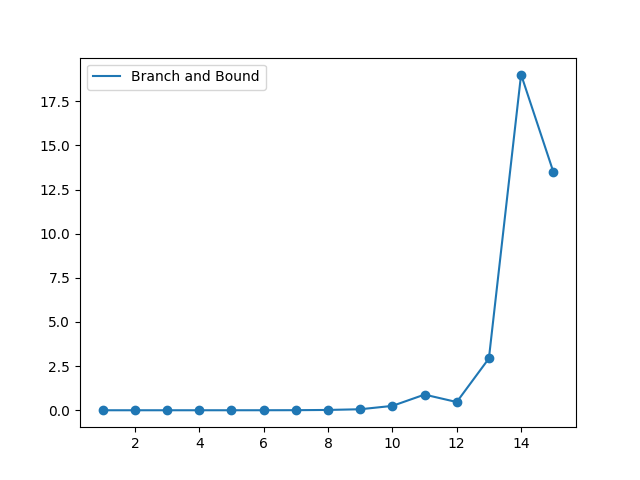
\includegraphics[scale=1]{../../graphics/branch_and_bound.png}
\end{figure}

Aquí vemos una gráfica del tiempo de ejecución en función del tamaño, y como era de esperarse, cuando alcanzamos valores de $n$ superiores a 12, se produce un salto brusco en el tiempo de ejecución. Este se debe a que aunque el algoritmo branch and bound sea muy bueno, el orden del algoritmo sigue siendo $O(n!)$.

\end{document}